\documentclass[11pt, a4paper]{article}
\usepackage{pdfpages}
\usepackage{parallel}
\usepackage[T2A]{fontenc}
\usepackage{ucs}
\usepackage[utf8x]{inputenc}
\usepackage[polish,english,russian]{babel}
\usepackage{hyperref}
\usepackage{rotating}
\usepackage[inner=2cm,top=1.8cm,outer=2cm,bottom=2.3cm,nohead]{geometry}
\usepackage{listings}
\usepackage{graphicx}
\usepackage{wrapfig}
\usepackage{longtable}
\usepackage{indentfirst}
\usepackage{array}
\usepackage{tikzsymbols}
\usepackage{soul}
\usepackage[ruled,vlined]{algorithm2e}
%\counterwithout{figure}{section} 

\usepackage{url}
\makeatletter
\g@addto@macro{\UrlBreaks}{\UrlOrds}
\makeatother

\newcolumntype{P}[1]{>{\raggedright\arraybackslash}p{#1}}
\frenchspacing
\usepackage{fixltx2e} %text sub- and superscripts
\usepackage{icomma} % коскі ў матэматычным рэжыме
\PreloadUnicodePage{4}

\newcommand{\longpage}{\enlargethispage{\baselineskip}}
\newcommand{\shortpage}{\enlargethispage{-\baselineskip}}

\def\switchlang#1{\expandafter\csname switchlang#1\endcsname}
\def\switchlangbe{
\let\saverefname=\refname%
\def\refname{Літаратура}%
\def\figurename{Іл.}%
}
\def\switchlangen{
\let\saverefname=\refname%
\def\refname{References}%
\def\figurename{Fig.}%
}
\def\switchlangru{
\let\saverefname=\refname%
\let\savefigurename=\figurename%
\def\refname{Литература}%
\def\figurename{Рис.}%
}

\hyphenation{admi-ni-stra-tive}
\hyphenation{ex-pe-ri-ence}
\hyphenation{fle-xi-bi-li-ty}
\hyphenation{Py-thon}
\hyphenation{ma-the-ma-ti-cal}
\hyphenation{re-ported}
\hyphenation{imp-le-menta-tions}
\hyphenation{pro-vides}
\hyphenation{en-gi-neering}
\hyphenation{com-pa-ti-bi-li-ty}
\hyphenation{im-pos-sible}
\hyphenation{desk-top}
\hyphenation{elec-tro-nic}
\hyphenation{com-pa-ny}
\hyphenation{de-ve-lop-ment}
\hyphenation{de-ve-loping}
\hyphenation{de-ve-lop}
\hyphenation{da-ta-ba-se}
\hyphenation{plat-forms}
\hyphenation{or-ga-ni-za-tion}
\hyphenation{pro-gramming}
\hyphenation{in-stru-ments}
\hyphenation{Li-nux}
\hyphenation{sour-ce}
\hyphenation{en-vi-ron-ment}
\hyphenation{Te-le-pathy}
\hyphenation{Li-nux-ov-ka}
\hyphenation{Open-BSD}
\hyphenation{Free-BSD}
\hyphenation{men-ti-on-ed}
\hyphenation{app-li-ca-tion}

\def\progref!#1!{\texttt{#1}}
\renewcommand{\arraystretch}{2} %Іначай формулы ў матрыцы зліпаюцца з лініямі
\usepackage{array}

\def\interview #1 (#2), #3, #4, #5\par{

\section[#1, #3, #4]{#1 -- #3, #4}
\def\qname{LVEE}
\def\aname{#1}
\def\q ##1\par{{\noindent \bf \qname: ##1 }\par}
\def\a{{\noindent \bf \aname: } \def\qname{L}\def\aname{#2}}
}

\def\interview* #1 (#2), #3, #4, #5\par{

\section*{#1\\{\small\rm #3, #4. #5}}
\ifx\ParallelWhichBox\undefined%
    \addcontentsline{toc}{section}{#1, #3, #4}%
\else%
\ifnum\ParallelWhichBox=0%
    \addcontentsline{toc}{section}{#1, #3, #4}%
\fi\fi%

\def\qname{LVEE}
\def\aname{#1}
\def\q ##1\par{{\noindent \bf \qname: ##1 }\par}
\def\a{{\noindent \bf \aname: } \def\qname{L}\def\aname{#2}}
}

\newcommand{\interviewfooter}[1]{
\vskip 1em
\noindent \textit{#1}
}


\begin{document}

\title{1998 "--- Apple Puck Mouse}
\date{}
\maketitle
Мышь Apple USB mouse, часто называемая <<шайбой>> (англ. <<puck>>)  из-за своей необычной формы, была разработана компанией Apple в 1998 году. Это была первая коммерчески выпущенная мышь Apple mouse, которая использовала формат подключения USB, а не шину Apple ADB. Многие обозреватели критиковали данную мышь за ее недостаточно эргономичный дизайн.

\begin{figure}[h]
    \centering
    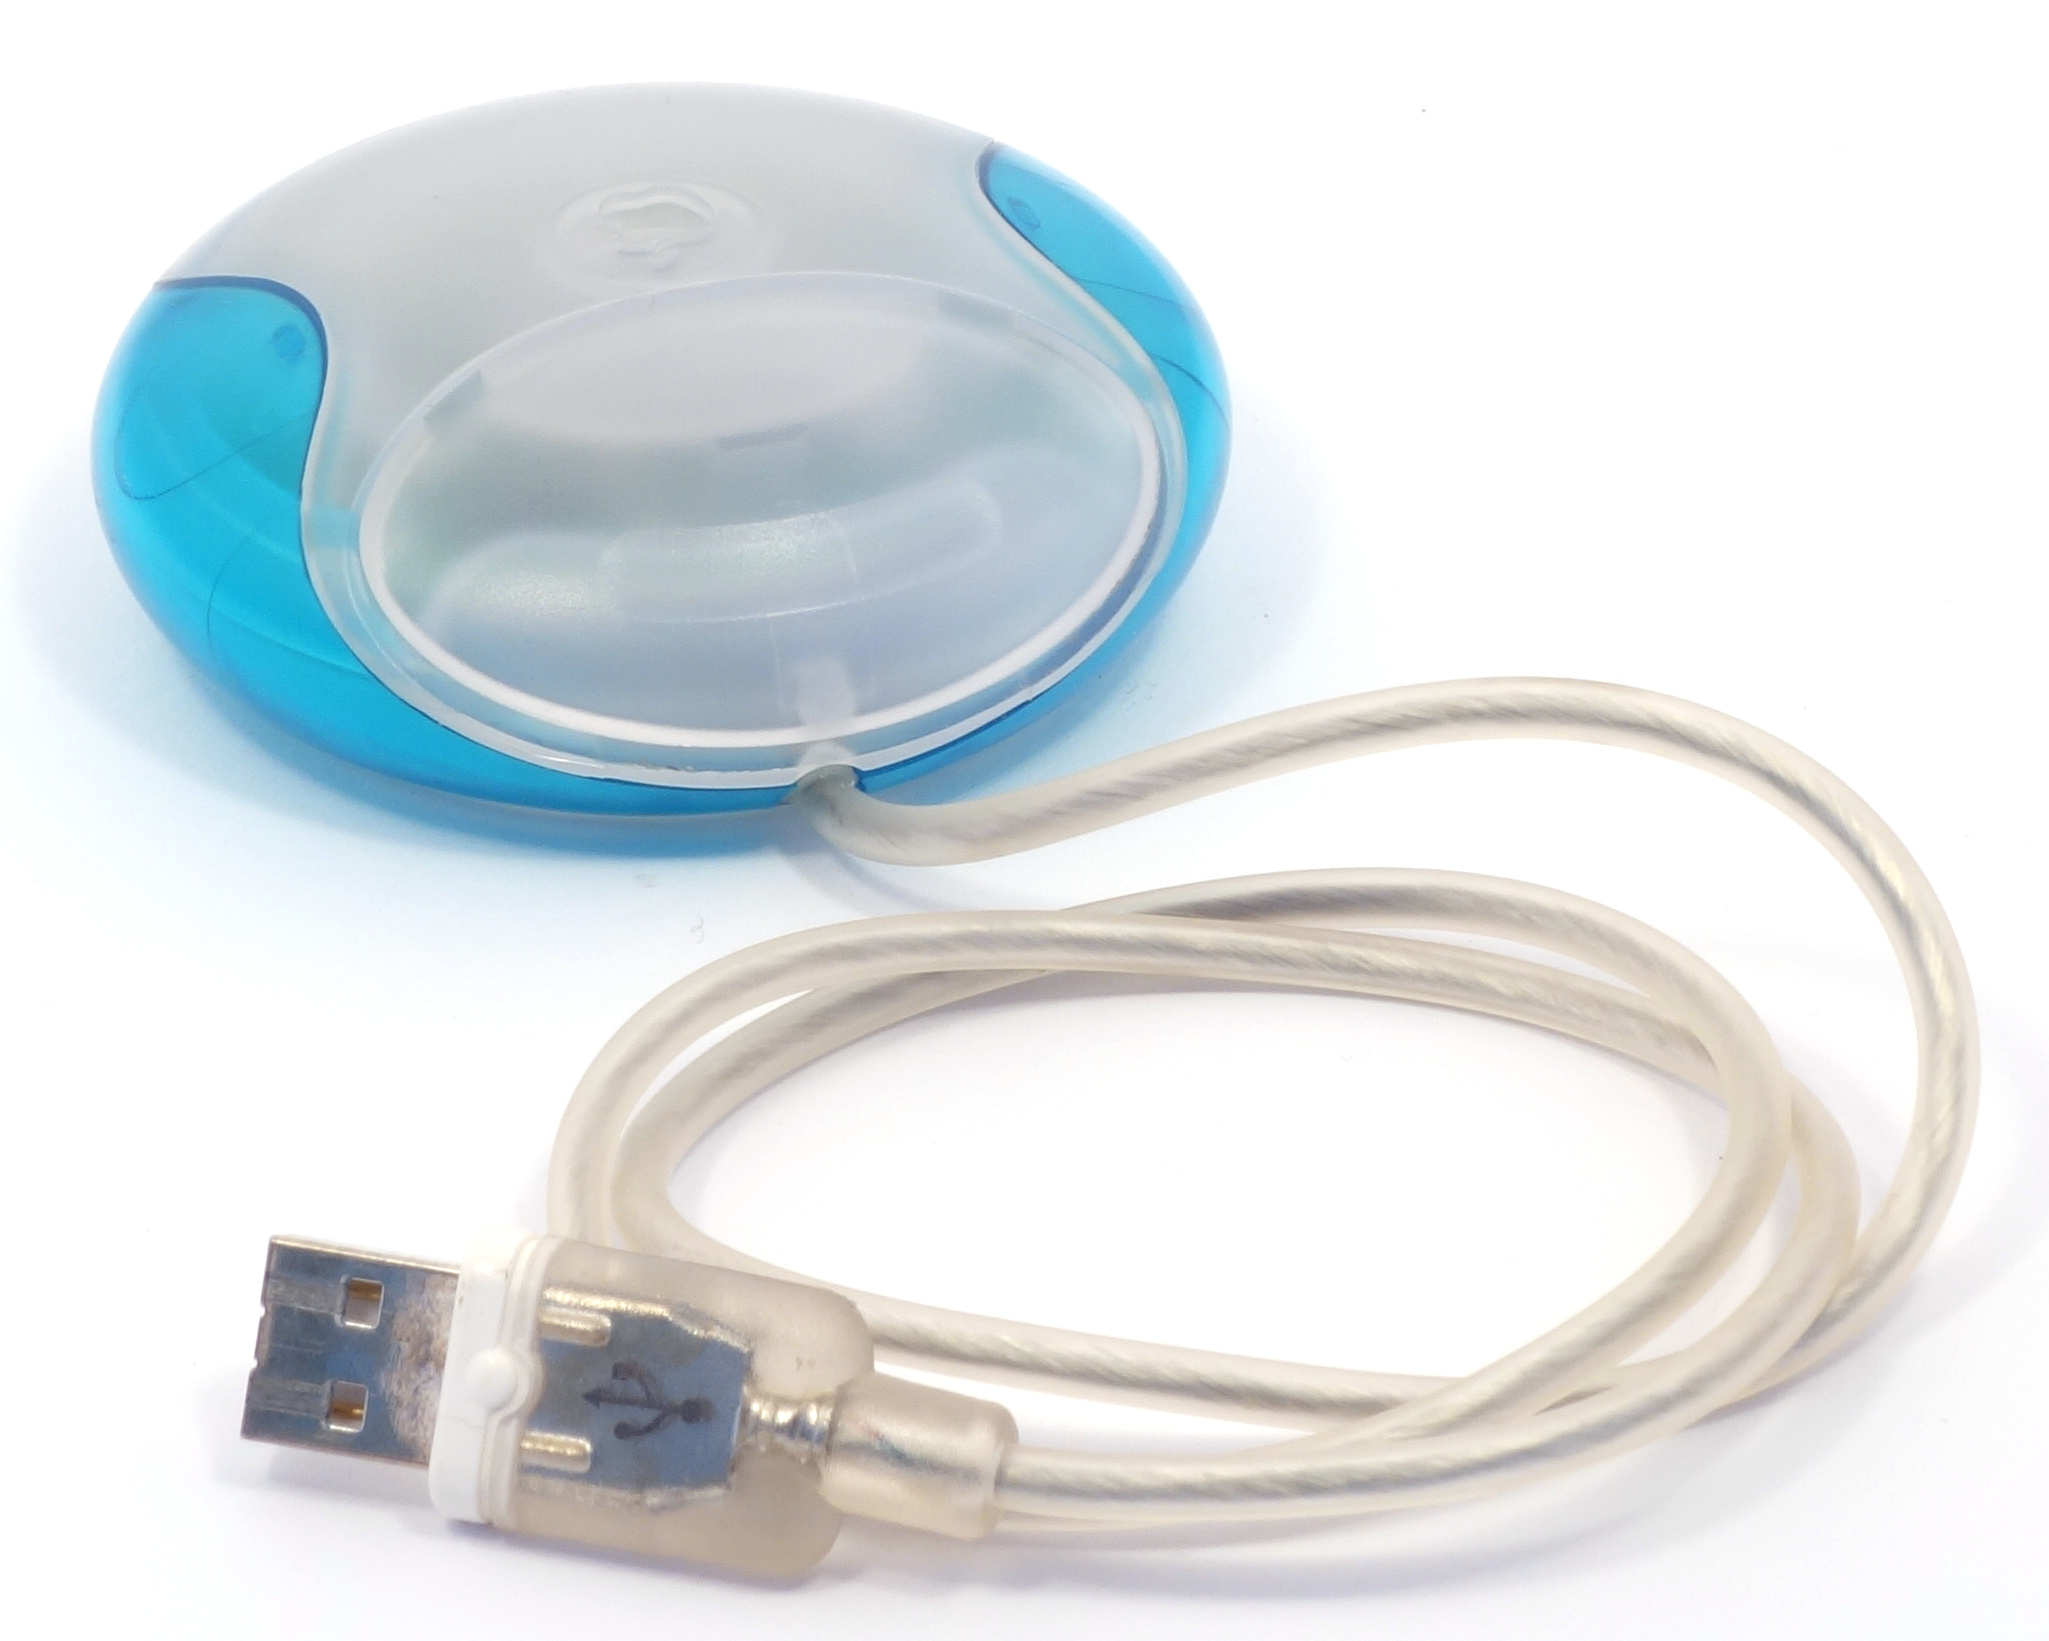
\includegraphics[scale=0.8]{1998_apple_puck/apple60.jpg}
    \caption{Apple Puck Mouse}
    \label{fig:pic}
\end{figure}

В отличие от большинства манипуляторов, эта мышь имеет круглую форму, и у нее есть одна кнопка, расположенная вверху, как и у предыдущих мышей Apple. При этом мышь имеет зазор между кнопкой и корпусом, показывающий, куда именно пользователь должен нажимать \cite{Apple}.

\begin{figure}[h]
    \centering
    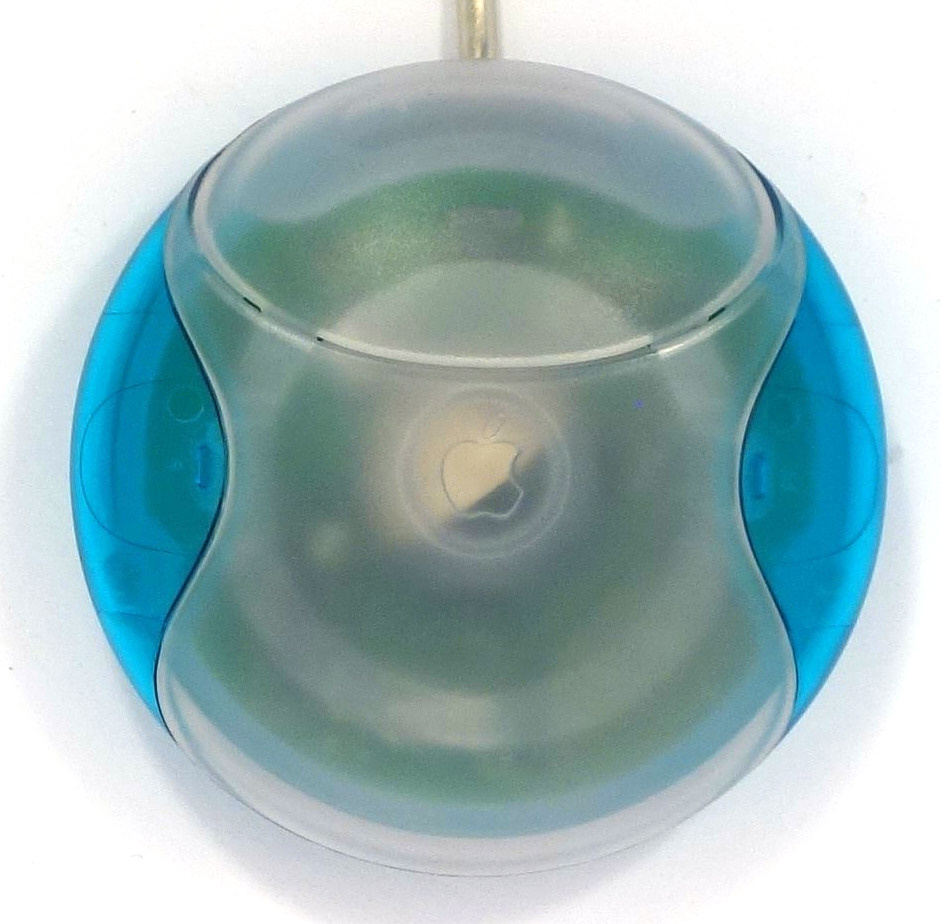
\includegraphics[scale=0.65]{1998_apple_puck/appleup60.jpg}
    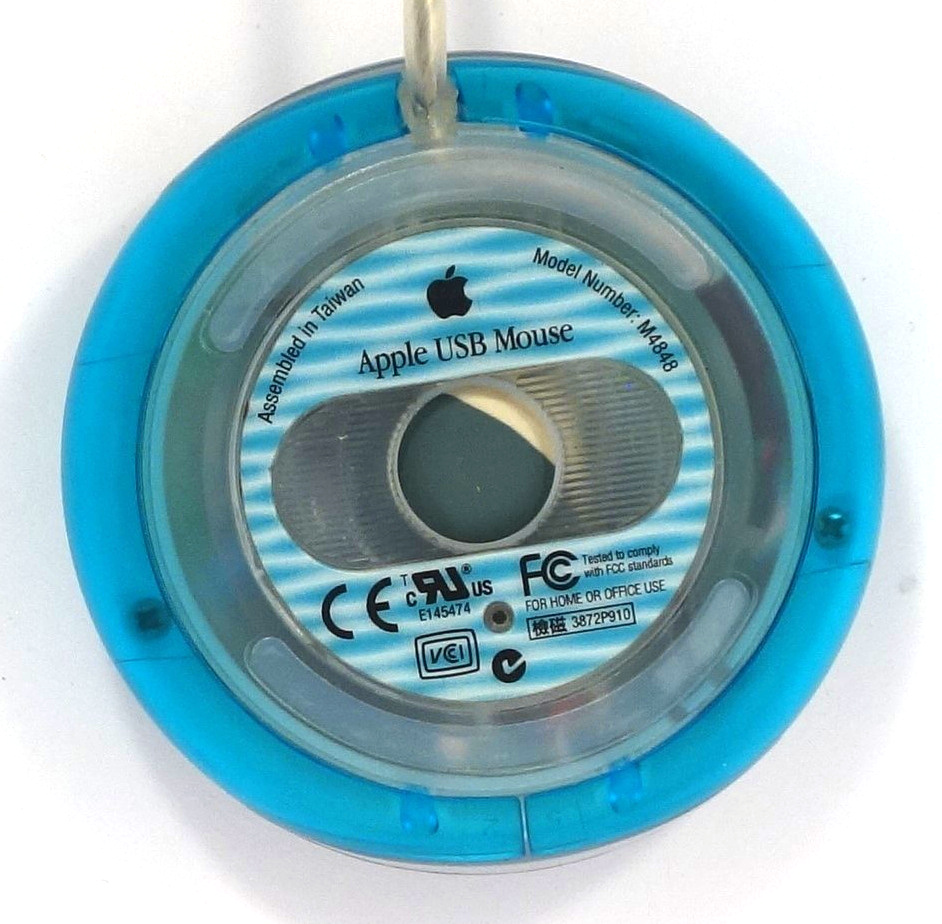
\includegraphics[scale=0.65]{1998_apple_puck/appledown60.jpg}
    \caption{Apple Puck Mouse, вид сверху и снизу}
    \label{fig:top}
\end{figure}

Круглая форма мыши была признана сообществом неудобной из-за небольшого размера данного конкретного манипулятора и склонности вращаться при использовании.
Также из-за малого размера, перемещение мыши на самом деле требовало гораздо большего количества движений  пальцев и  меньшего количества движений запястья по сравнению с более крупными мышами (рис. \ref{fig:size}, \ref{fig:hand}).

\begin{figure}[h]
    \centering
    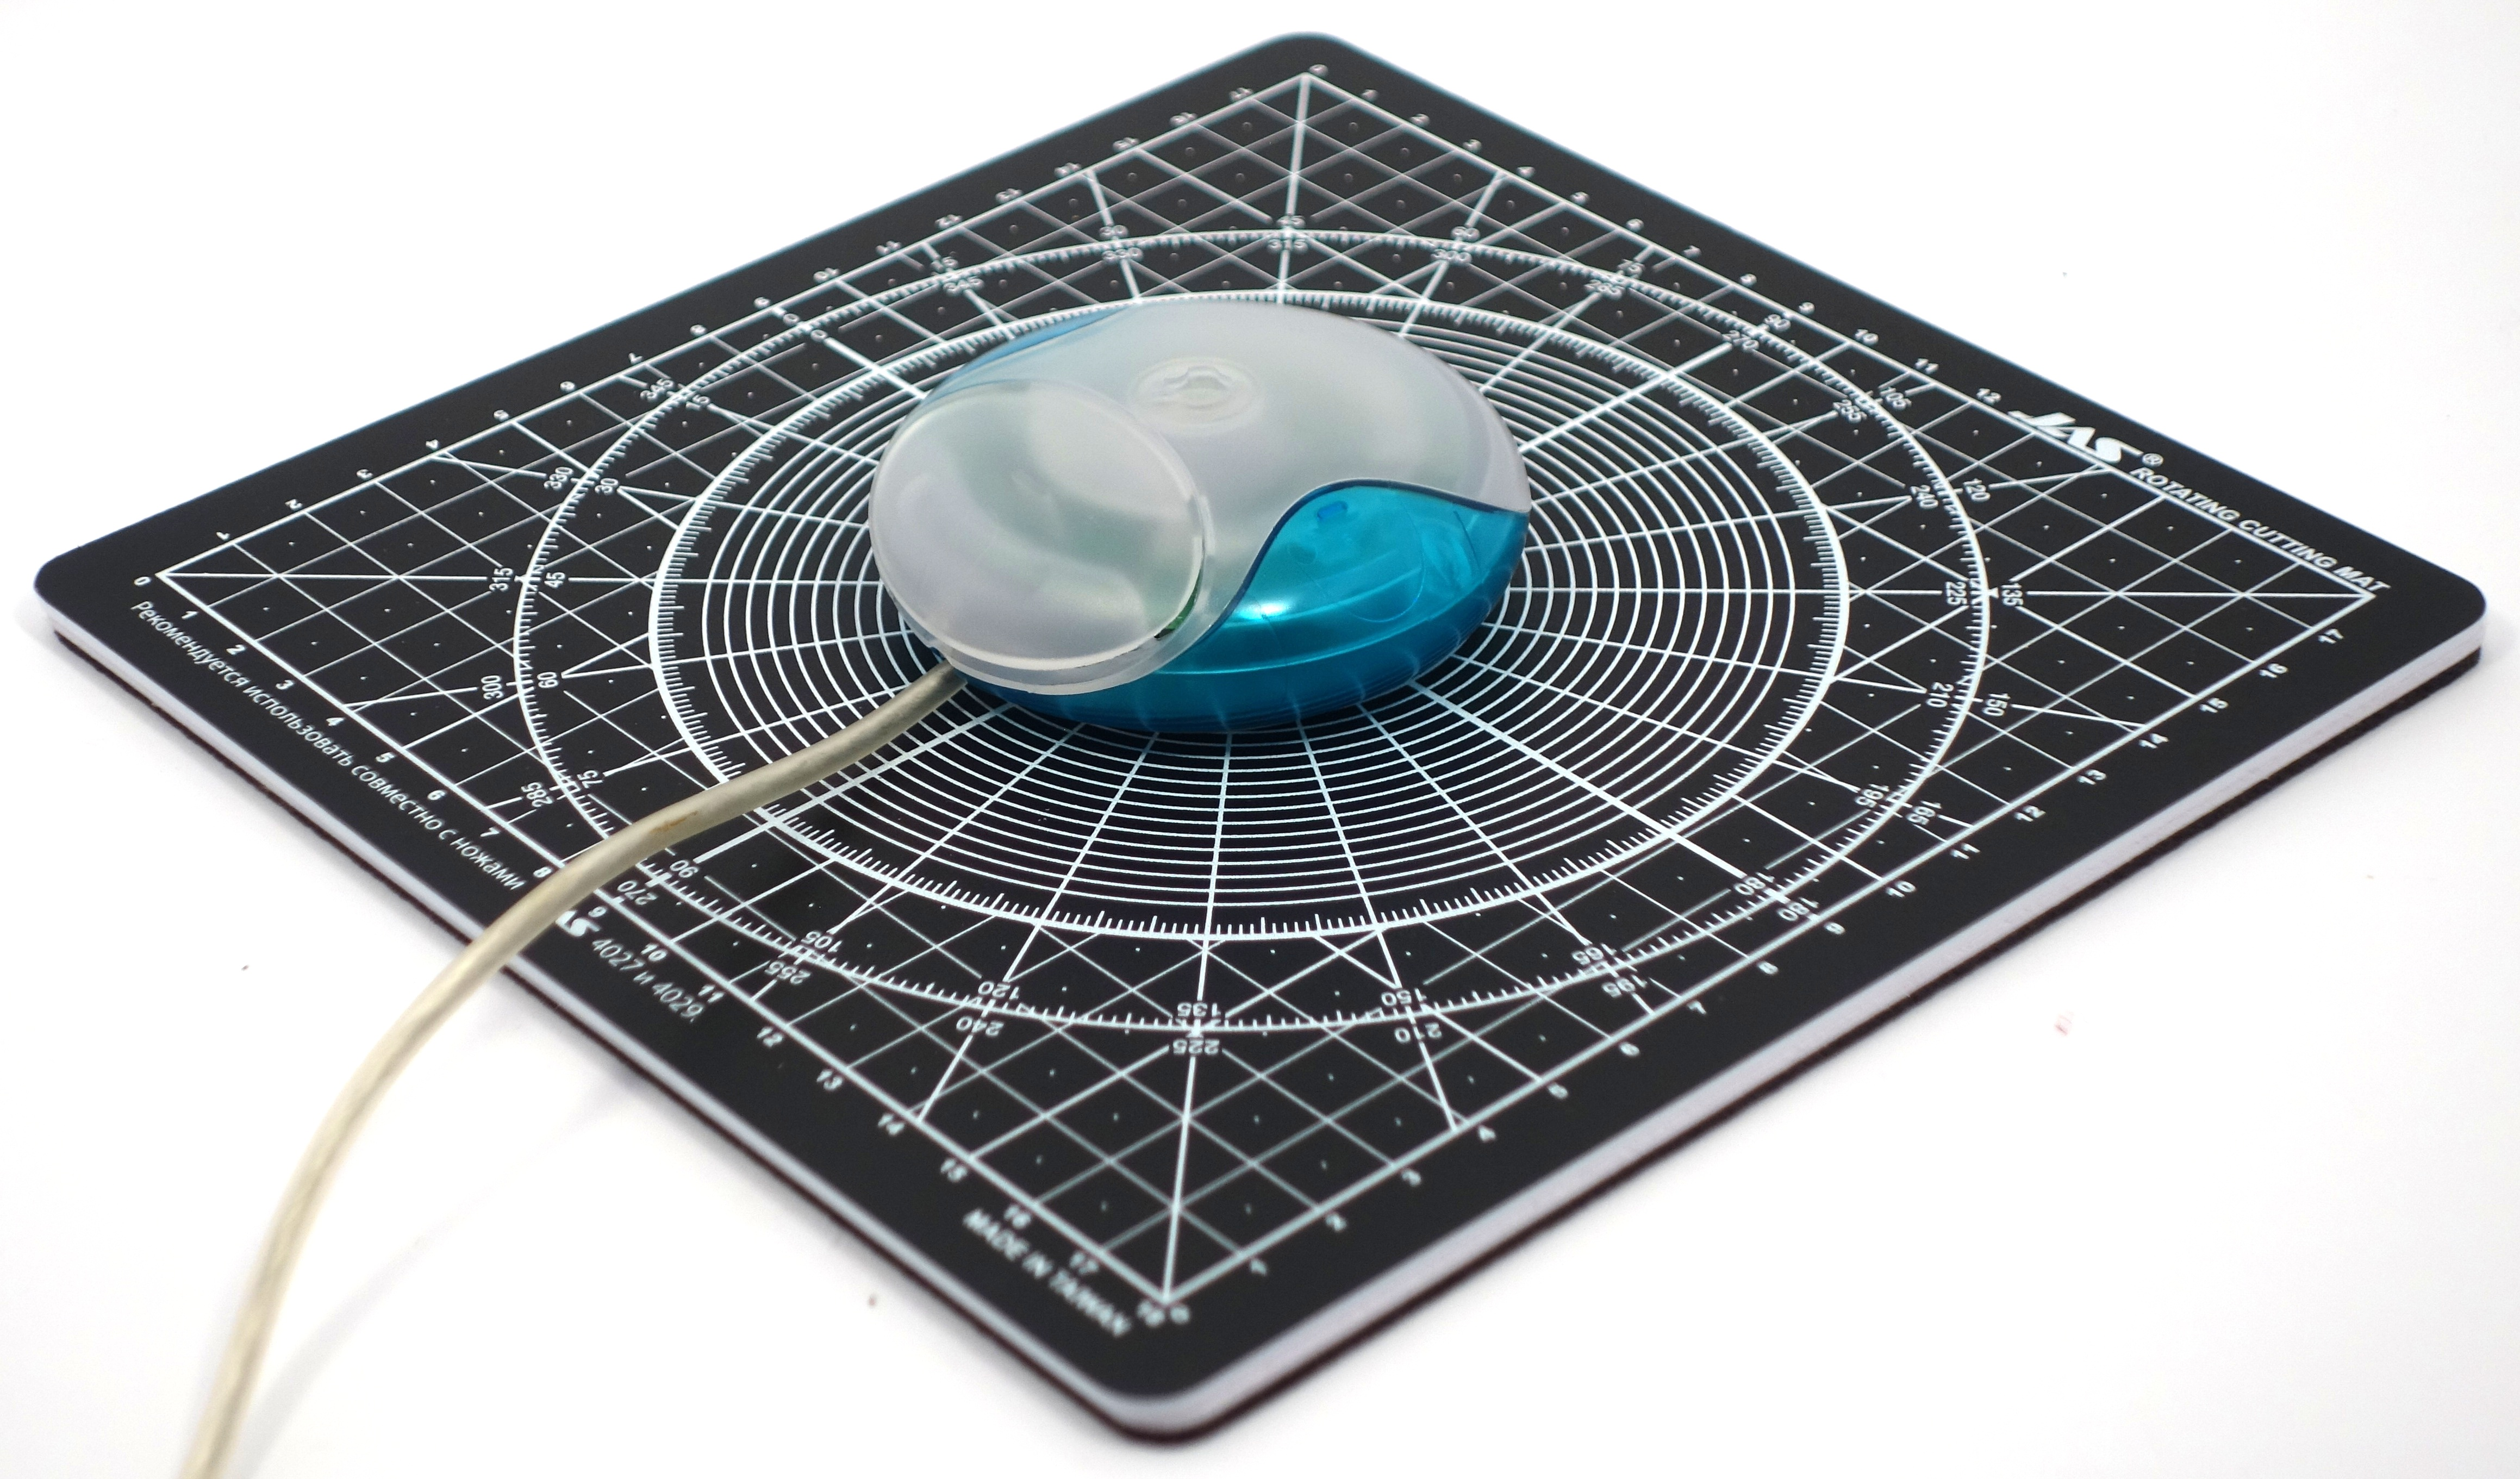
\includegraphics[scale=0.4]{1998_apple_puck/appleset60.jpg}
    \caption{Apple Puck Mouse на размерном коврике с шагом сетки 1~см}
    \label{fig:size}
\end{figure}

\begin{figure}[h]
    \centering
    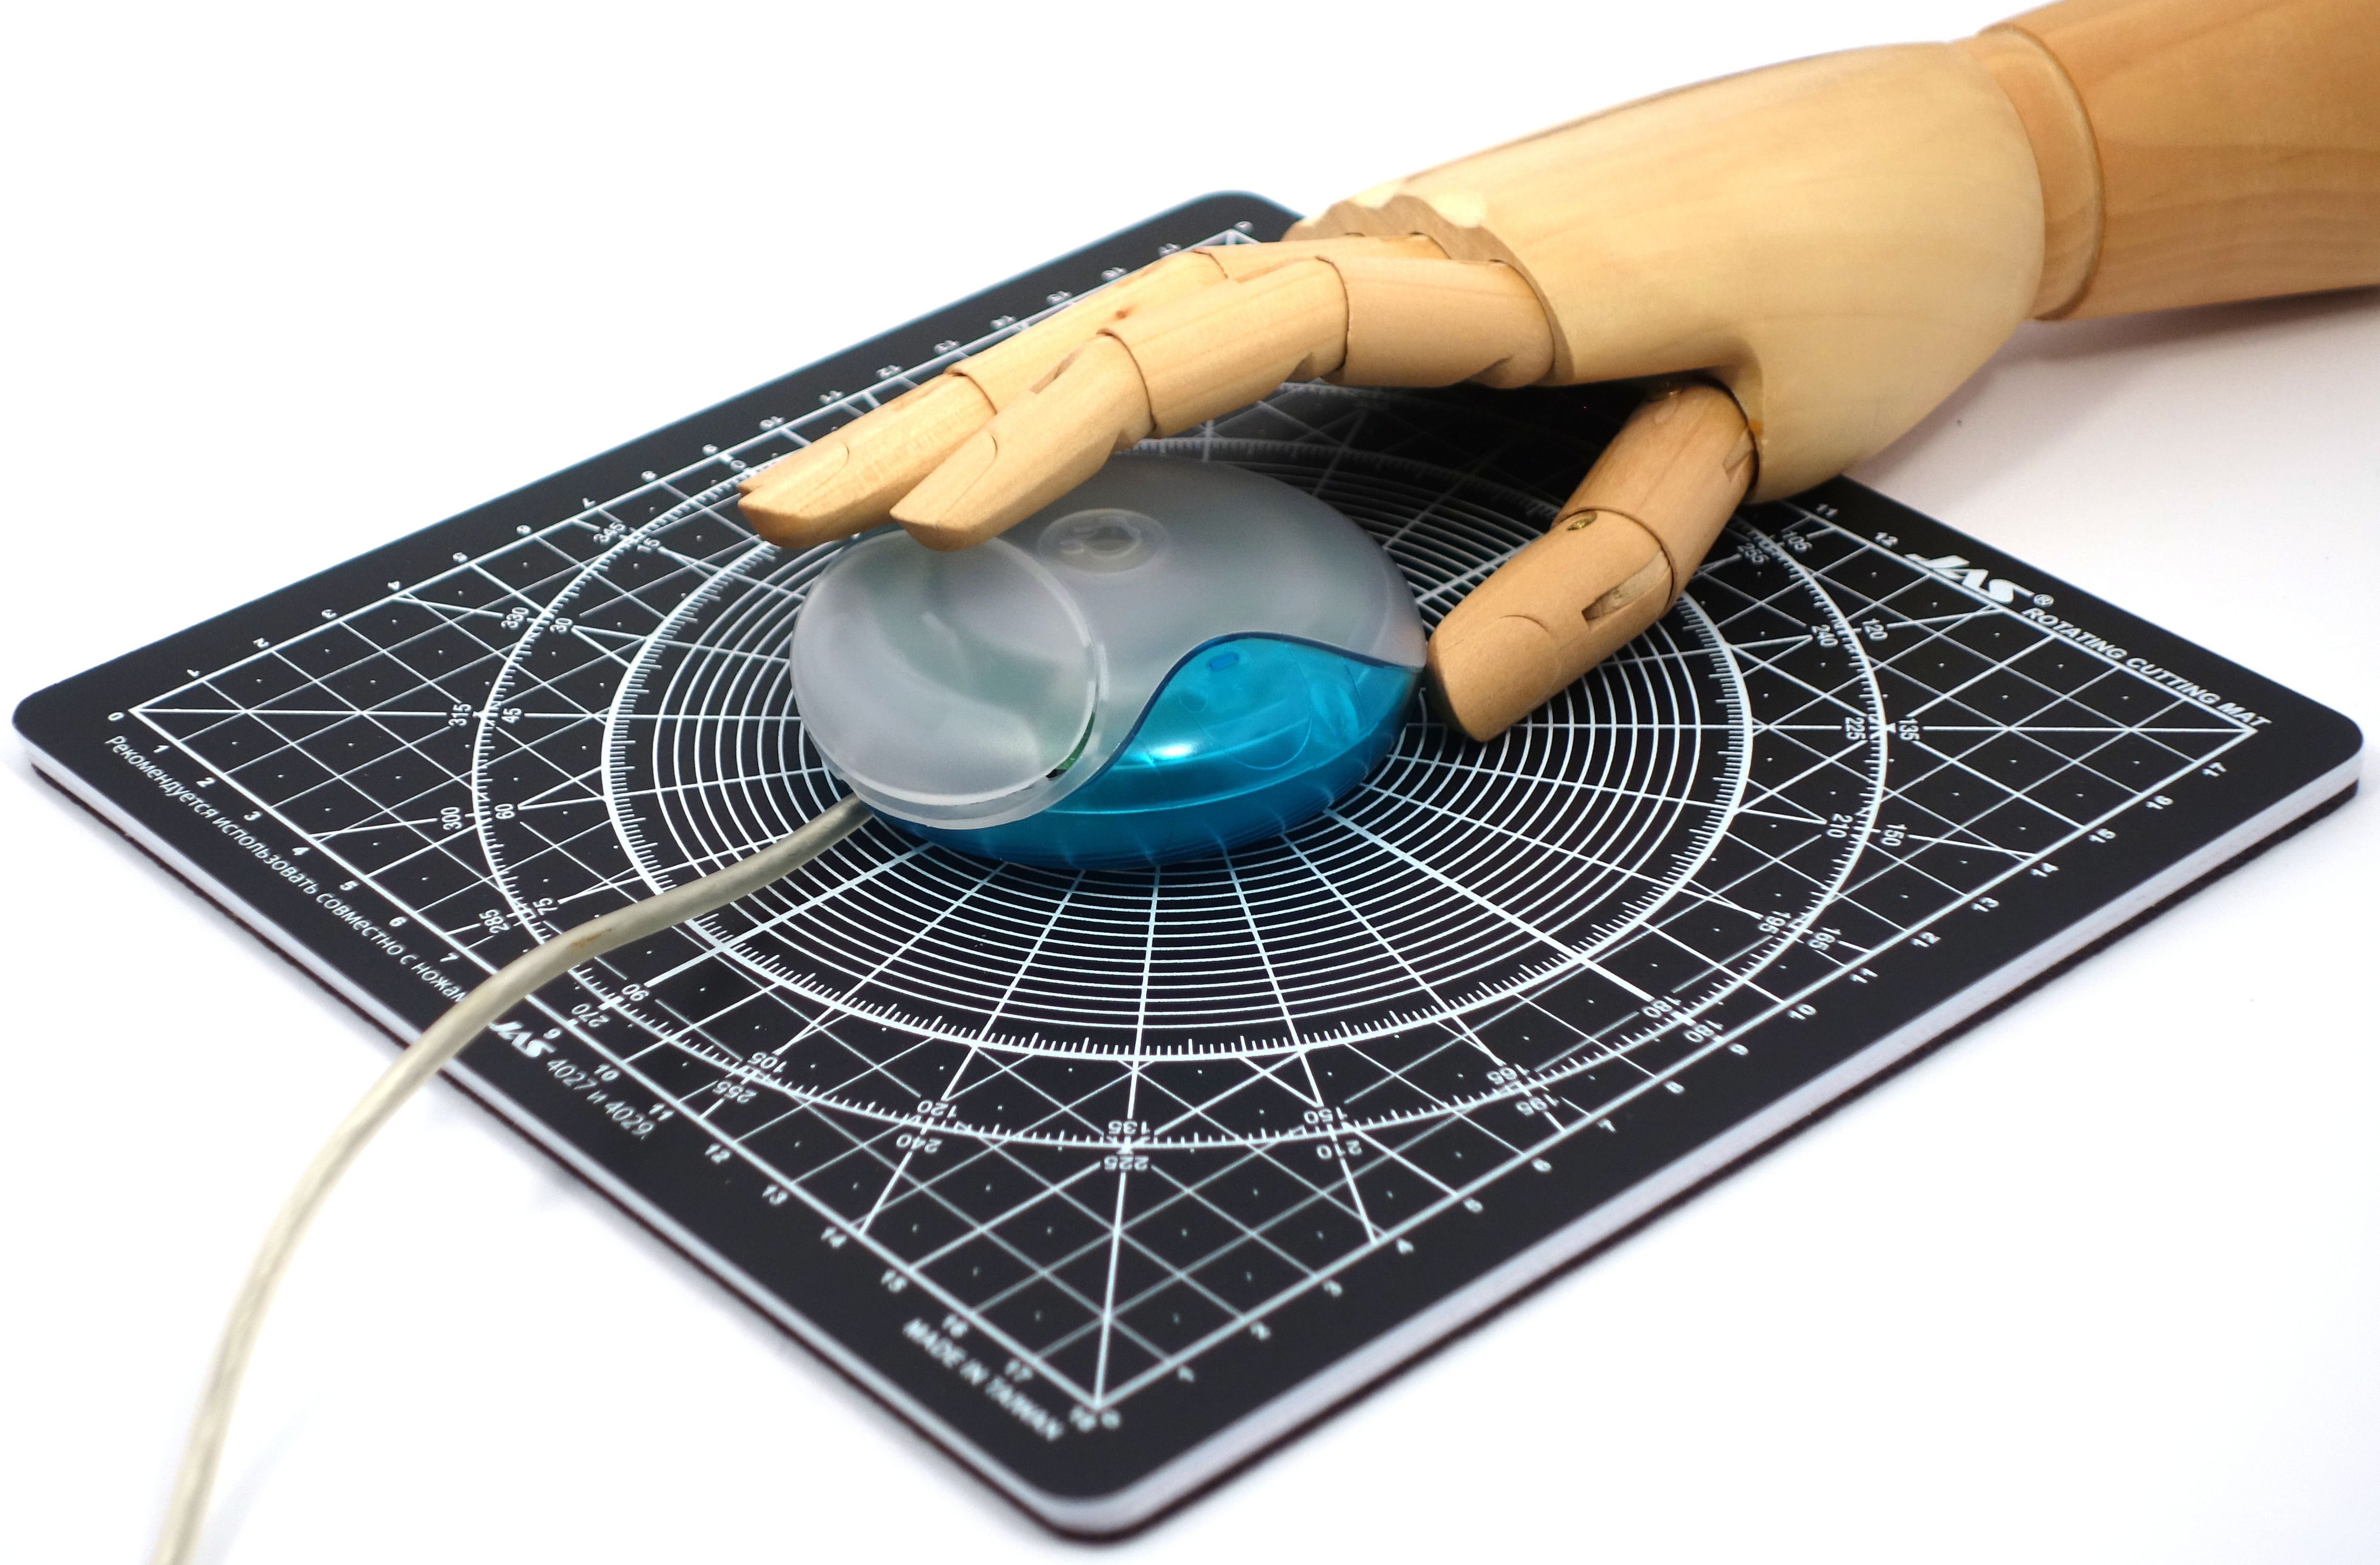
\includegraphics[scale=0.4]{1998_apple_puck/appleset62.jpg}
    \caption{Apple Puck Mouse с моделью руки человека}
    \label{fig:hand}
\end{figure}

Это стало основной причиной успеха адаптеров-накладок, таких как iCatch Mouse Adapter \cite{icatch}, придававших мыши более продолговатую форму (рис. \ref{fig:addon}).

\begin{figure}[h]
    \centering
    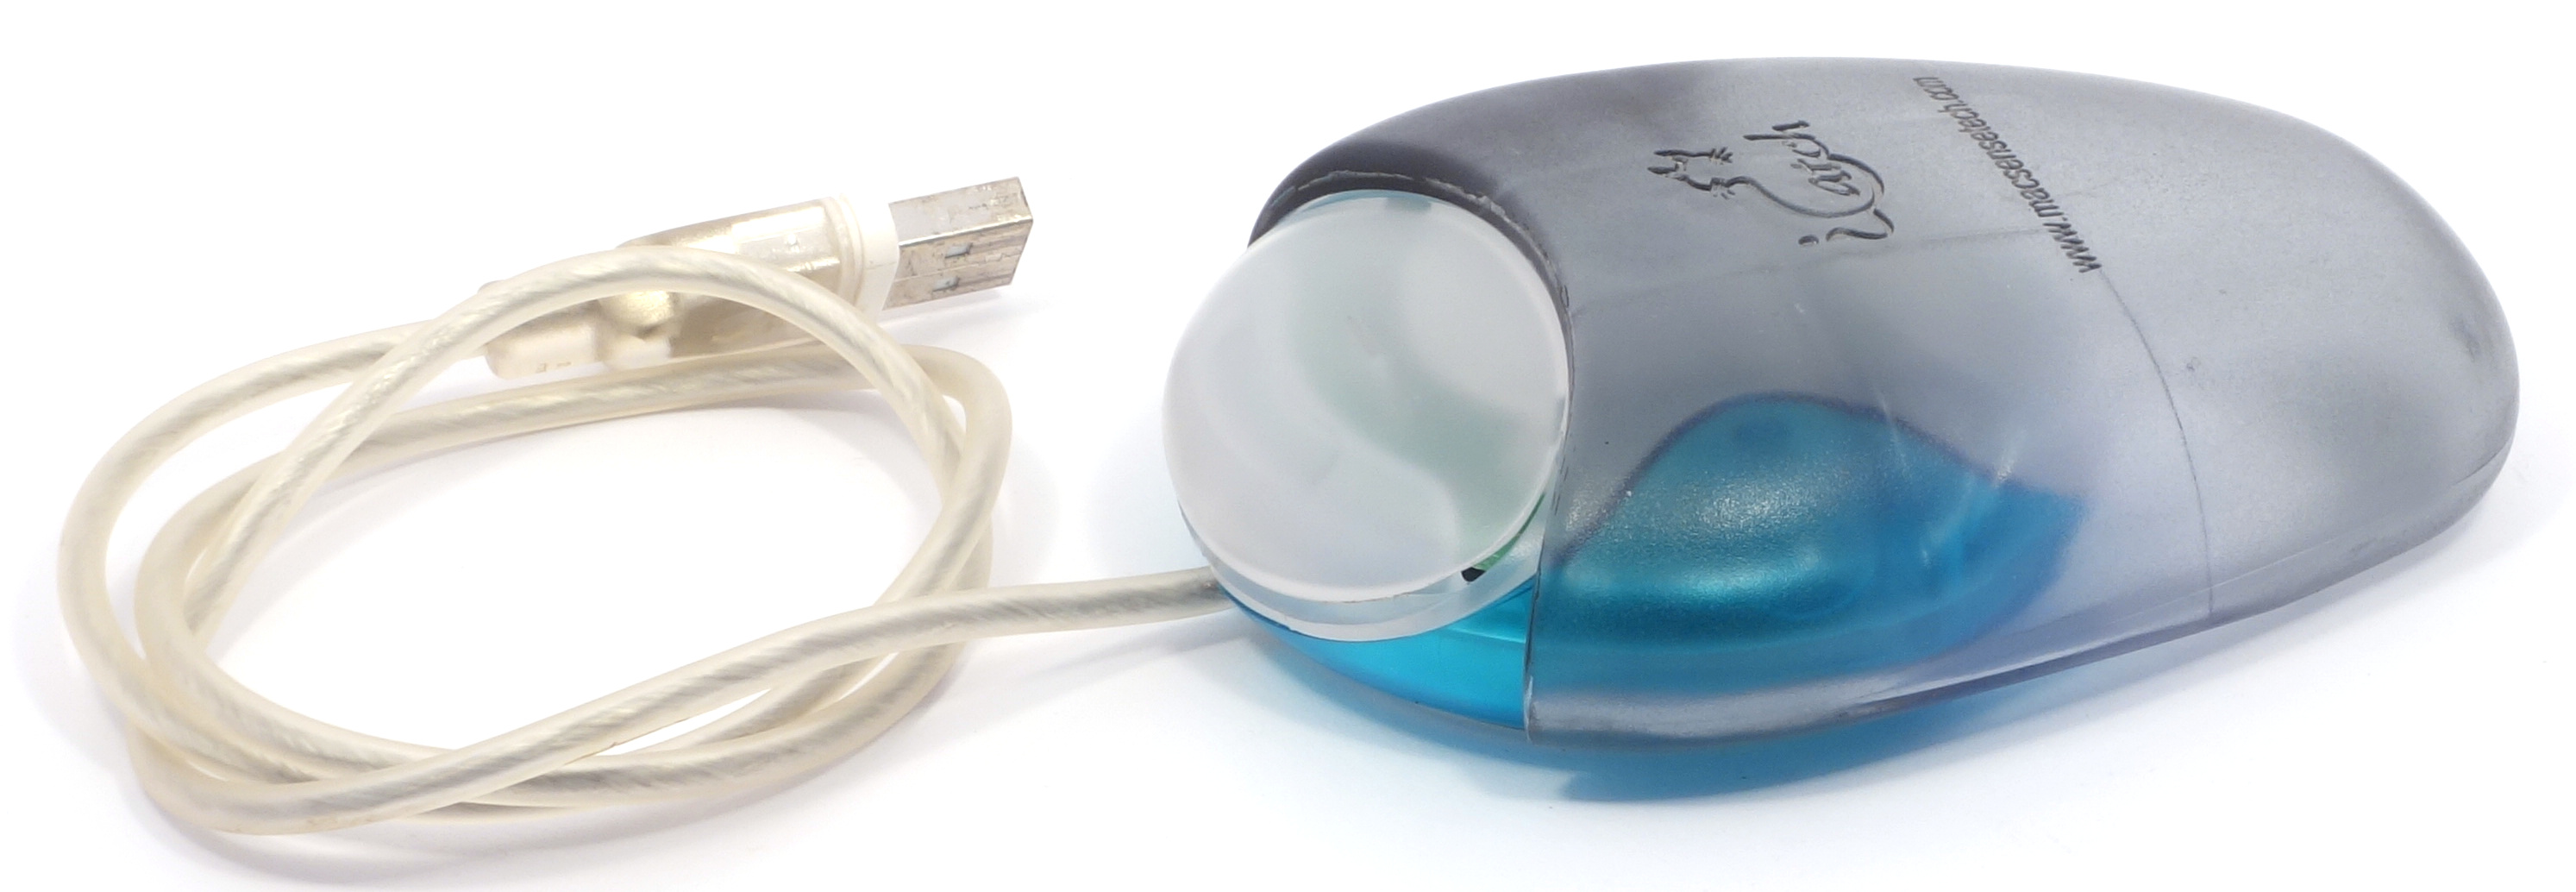
\includegraphics[scale=0.45]{1998_apple_puck/apple63.jpg}
    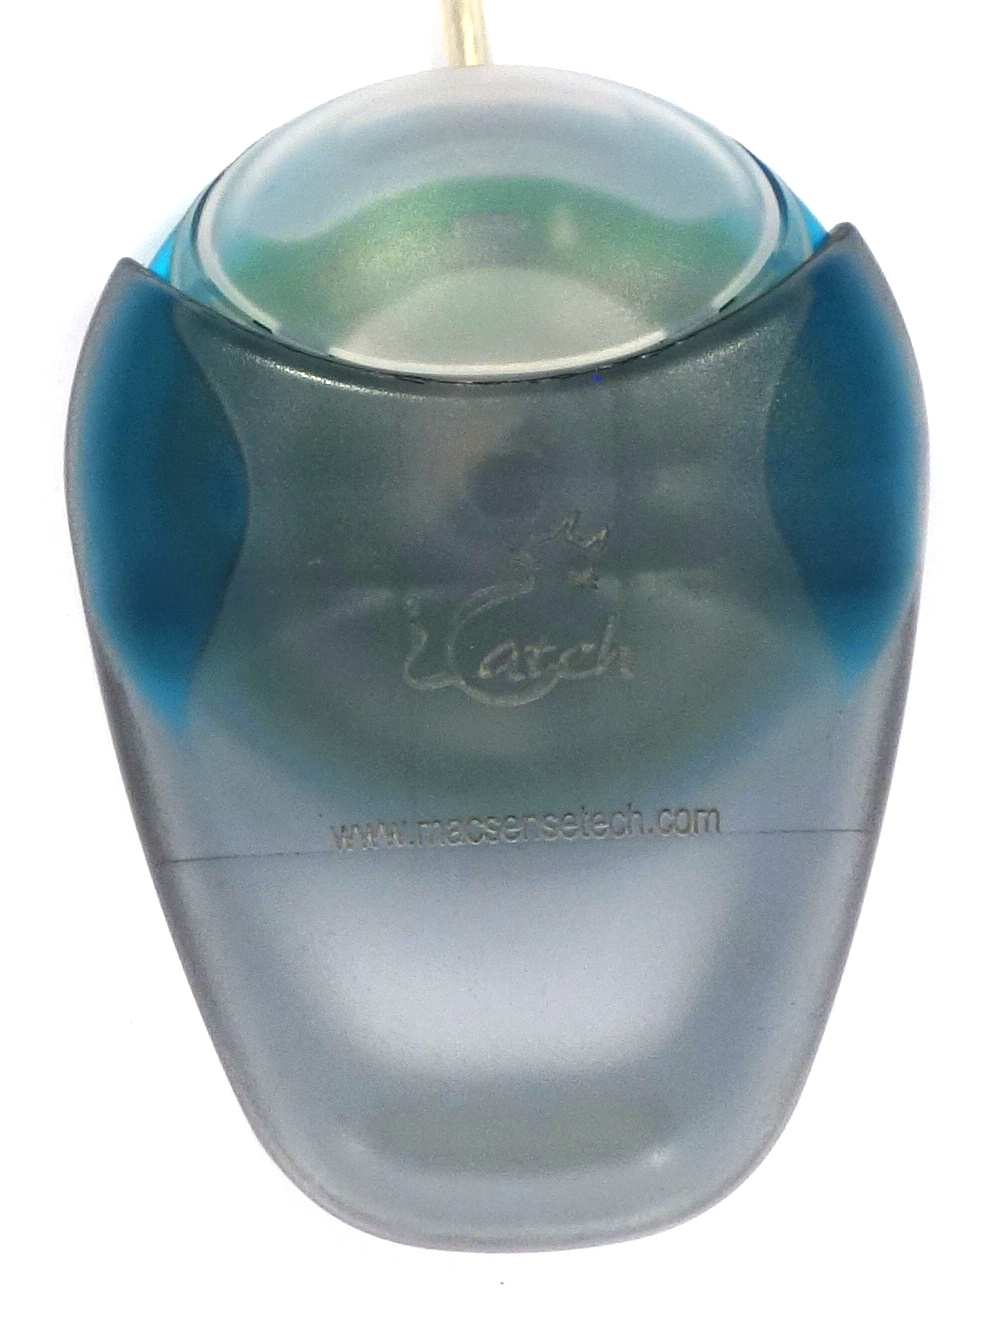
\includegraphics[scale=0.45]{1998_apple_puck/appleup63.JPG}
    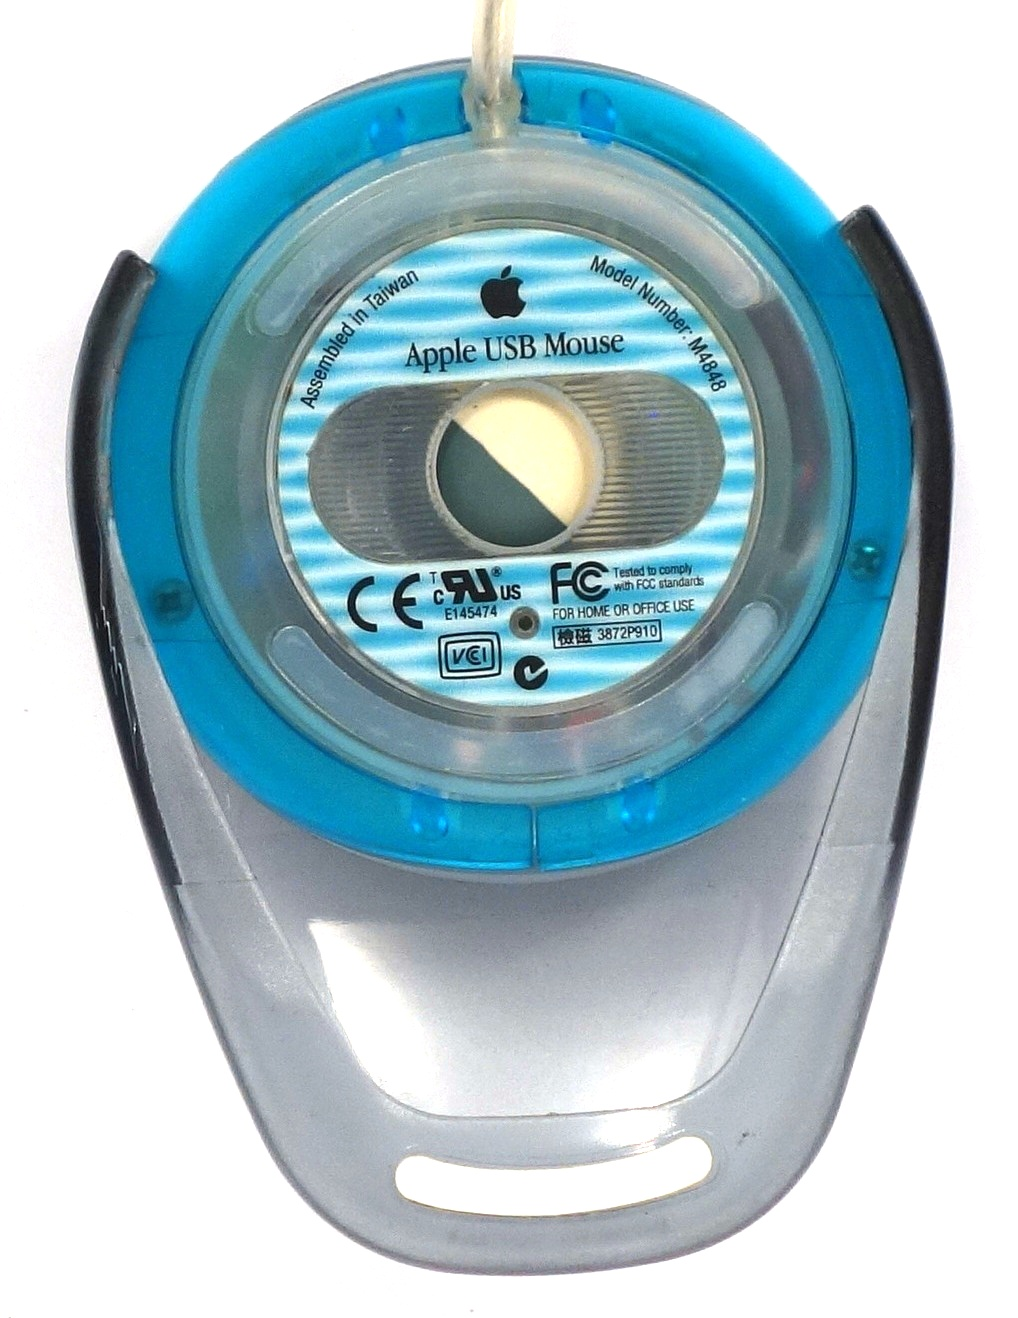
\includegraphics[scale=0.45]{1998_apple_puck/appledown63.JPG}
    \caption{Apple Puck Mouse, вид с накладкой}
    \label{fig:addon}
\end{figure}



В полупрозрачном пластике помещалась печатная плата и двухцветный шар, который можно было легко разглядеть. 


Однако идеально круглое тело часто приводило к ошибкам, так как пользователи предполагали, что мышь была в правильной ориентации, даже если это было не так. Позже Apple добавила ямочку на корпусе мыши, чтобы помочь пользователям почувствовать, в каком направлении указывала мышь.
\begin{figure}[h]
    \centering
    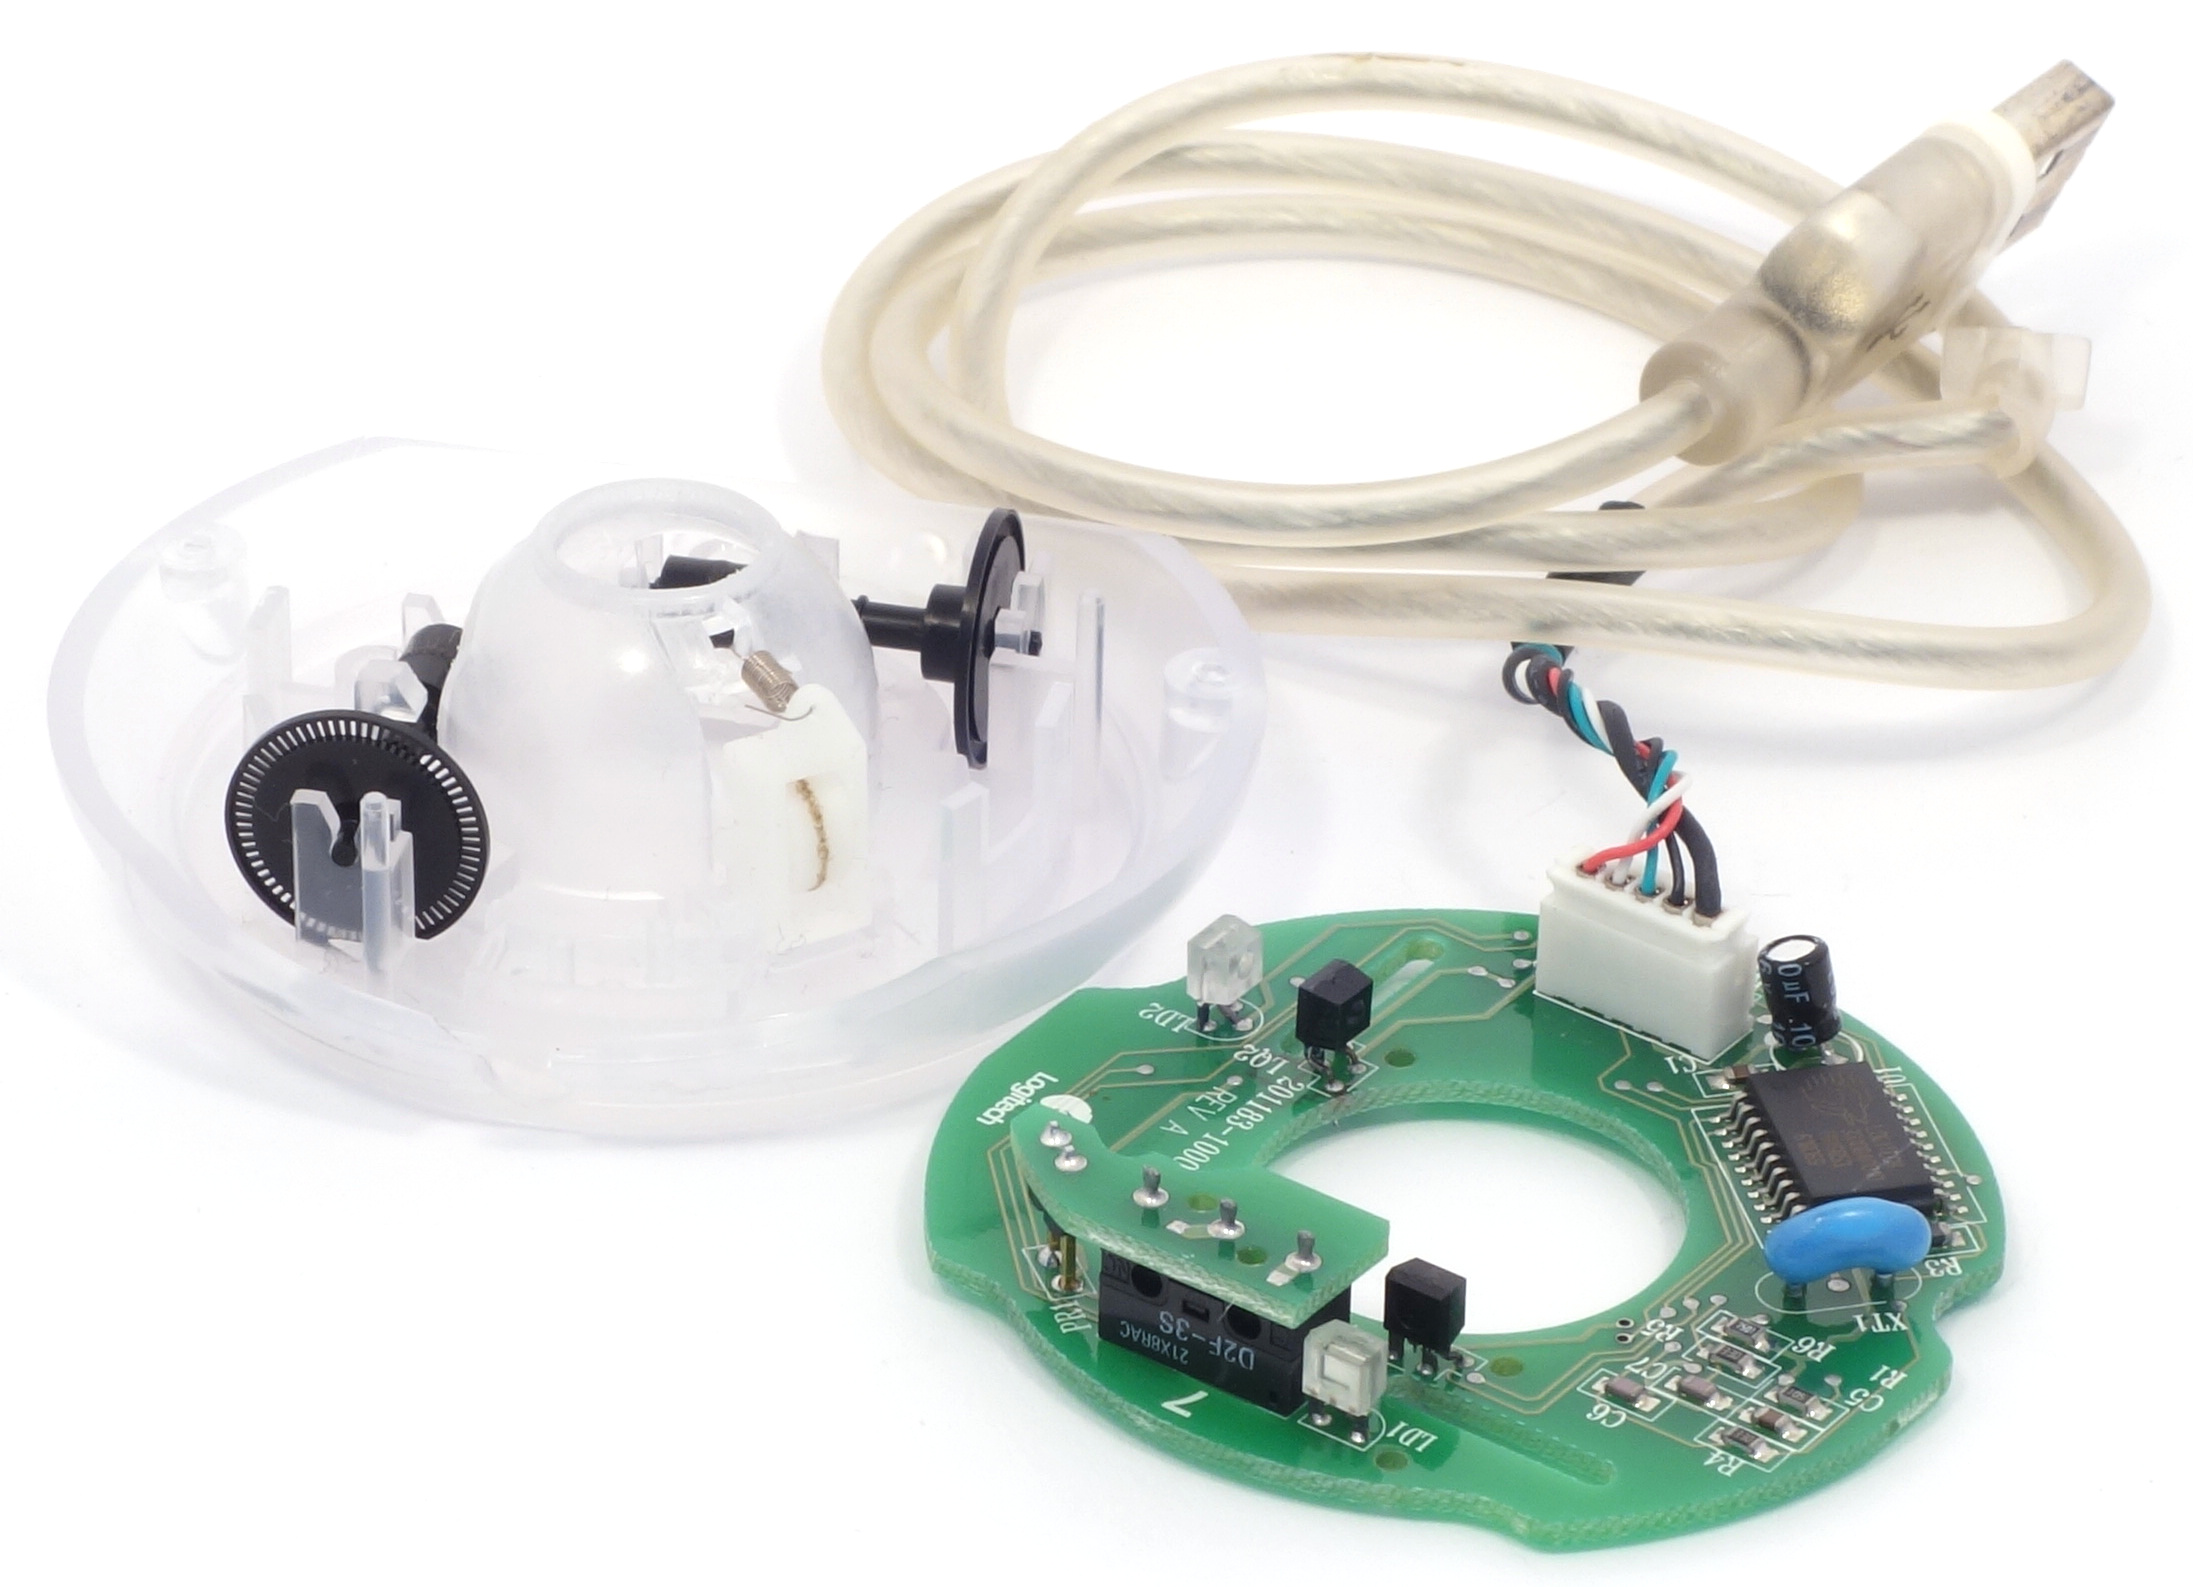
\includegraphics[scale=0.6]{1998_apple_puck/apple62.jpg}
    \caption{Apple Puck Mouse, в разобранном виде}
    \label{fig:inside}
\end{figure}

Внутреннее устройство данной мыши показано на рис. \ref{fig:inside}, что позволяет классифицировать  ее как оптомеханическую.

\begin{thebibliography}{9}

    \bibitem {Apple} An ode to the puck, Apple's first USB mouse "--- \url{https://thehouseofmoth.com/an-ode-to-the-puck-apples-first-usb-mouse/} 
    \bibitem{icatch} The iCatch Mouse Adapter \url{https://web.archive.org/web/20001024170633/http://www.macsensetech.com:80/Product/iCatch.html}
\end{thebibliography}

\end{document}
